\chapter{Badania} \label{przeg}
W tym rozdziale opisano przeprowadzone na kodzie badania. Zaczęto od opisania konkretnych problemów którymi się zajmowano, a następnie przeprowadzono badania mające potwierdzić czy algorytmy działają poprawnie. Na koniec przebadano zachowanie zaimplementowane filtry pod różnymi kątami.
\section{Opis poszczególnych problemów}
W badaniach zajęto się dwoma problemami wyznaczania lokalizacji. Pierwszy polega na ustalenie pozycji robota na podstawie pomiaru odległości od ściany, drugi na ustalenie pozycji samolotu na podstawie pomiaru wysokości. W oby przypadkach znano mapę środowiska w którym się znajdowały.
\subsection{Robot w pomieszczeniu} \label{robot_w_pomieszczeniu_desc}
Stan robota w pomieszczeniu opisano czterema liczbami:
\begin{equation*}
	x = \{p_x,p_y,\theta,v\}
\end{equation*}
gdzie $p_x$ i $p_y$ to pozycja robota, $\theta$ jest jego orientacją, natomiast $v$ prędkością. Pomiar odległości od ściany był zawsze wykonywany w kierunku $\theta$, i był miał Gaussowski rozkład. Mapa jest kwadratowym pokojem o wymiarach $1000$ na $1000$ jednostek, wypełnionym kołami o różnych średnicach, oraz ograniczany prostymi. Na rysunku \ref{przykladowa_mapa_pokoju} przedstawiono przykładową mapę.\\
O ile nie będzie napisane inaczej, robot zaczynał na środku mapy, miał prędkość 10 jednostek na iterację, i skręcał w lewo o $0.1rad$ na krok. Faktyczna pozycja robota była oznaczana przez czerwoną kropkę, estymowana pozycja przez żółtą, natomiast cząstki oznaczano na niebiesko.
\begin{figure}[H]
	\begin{center}
		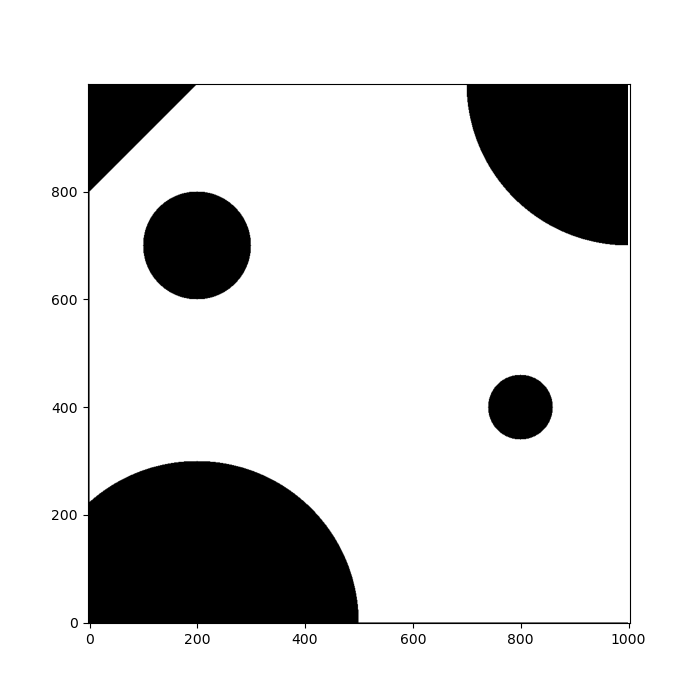
\includegraphics[width=10cm]{./przykladowa_mapa_pokoju.png}
		\caption{Przykładowa mapa pokoju}
		\label{przykladowa_mapa_pokoju}
	\end{center}
\end{figure}
\subsection{Samolot w locie}
Stan samolotu opisano tak samo jak stan robota w rozdziale \ref{robot_w_pomieszczeniu_desc}:
\begin{equation*}
	x = \{p_x,p_y,\theta,v\}
\end{equation*}
Mapa jest natomiast mapą wysokościową, w tym przypadku zdecydowano się na dwa warianty, pierwszy jest mapą fragmentu Wrocławia (przykład widoczny na rysunku \ref{przykladowa_mapa_wroclawia}), natomiast drugą wygenerowano jako szum, którego zmienność można kontrolować (przykład widoczny na rysunku \ref{przykladowa_mapa_szumu}).\\
O ile nie będzie napisane inaczej, samolot w lewym dolnym rogu mapy, miał prędkość 10 jednostek na iterację, i nie zmieniał orientacji $\theta=\frac{\pi}{4}$.
\begin{figure}[H]
	\begin{center}
		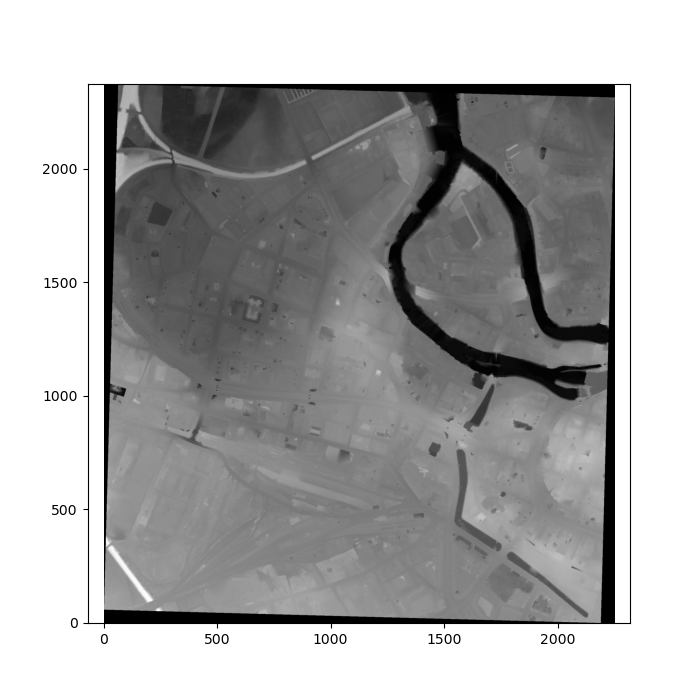
\includegraphics[width=10cm]{./przykladowa_mapa_wroclawia.png}
		\caption{Mapa wysokościowa fragmentu Wrocławia}
		\label{przykladowa_mapa_wroclawia}
	\end{center}
\end{figure}
\begin{figure}[H]
\begin{center}
	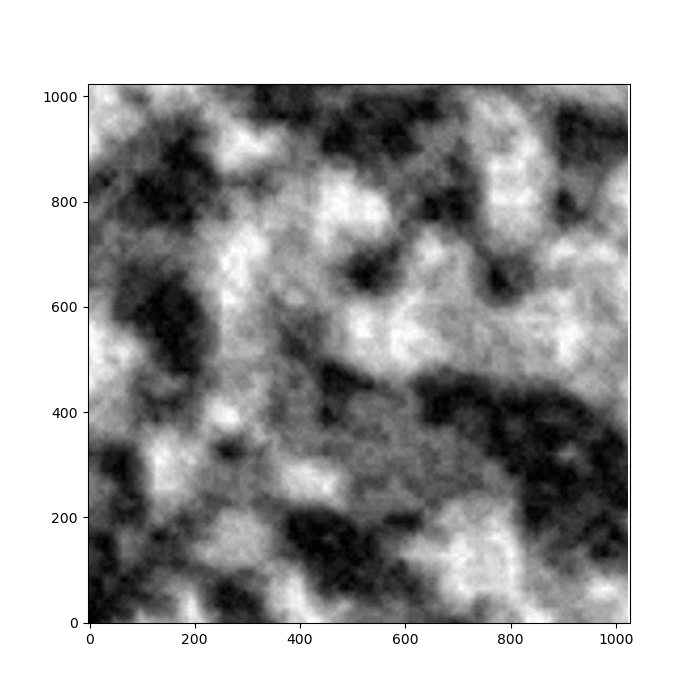
\includegraphics[width=10cm]{./przykladowa_mapa_szumu.png}
	\caption{Przykładowa mapa wysokościowa uzyskana z szumu}
	\label{przykladowa_mapa_szumu}
\end{center}
\end{figure}

\section{Badania poprawności działania}
W tym rozdziale zajęto się badaniami mającymi potwierdzić poprawne działanie zaimplementowanego rozwiązania. Na początku sprawdzono, jak zmiana generatora liczb losowych wpłynęła na wyniki, następnie sprawdzono, jak poradzi sobie algorytm przy braku punktów odniesienia, potem co się dzieje przy braku ewolucji systemu ($v=0$),
%a na koniec jak filtr radzi sobie z całkowicie losowymi pomiarami.
Nie skupiano się no konkretnych wartościach liczbowych, jedynie wizualnie oceniano wyniki.

\subsection{Wpływ generatora}
Przebadano trzy generatory wbudowane w język C++: domyślny linear congruential generator(LCG) \cite{lcg_wiki}, Mersenne Twister \cite{mersenne_wiki} oraz wbudowany niedeterministyczny generator. Populacja cząstek wynosiła $N=1000$. Wyniki rysowano po 1, 11 i 21 iteracjach filtra(nr iteracji oznaczano jako $k$). Wyniki przedstawiono na rysunkach \ref{lcg_example}, \ref{mersenne_example}, \ref{device_example}. Jak widać dla wszystkich generatorów wyniki są niemal takie same, i zbiegają do faktycznego położenia robota. Ponieważ dla każdego generatora uzyskano poprawne wyniki, w dalszych badaniach korzystano z generatora LCG ponieważ jest najprostszy, i, co za tym idzie, najszybszy.

\begin{figure}[H]
	\begin{center}
		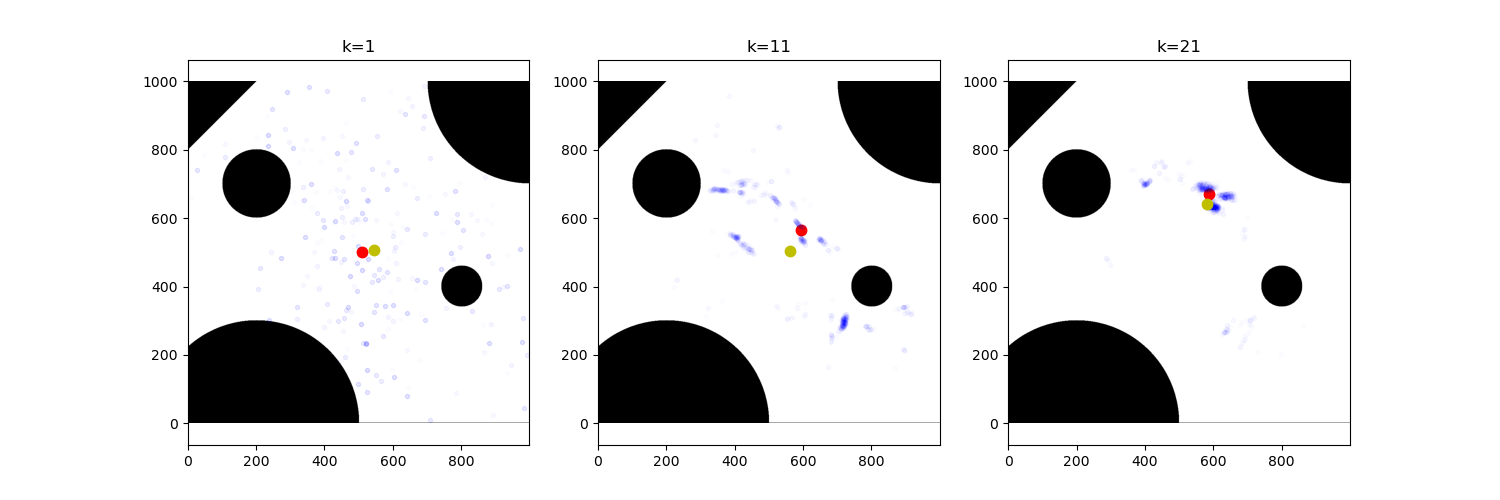
\includegraphics[width=15cm]{./lcg_example.png}
		\caption{Przykładowe wyniki dla generatora LCG}
		\label{lcg_example}
	\end{center}
\end{figure}

\begin{figure}[H]
	\begin{center}
		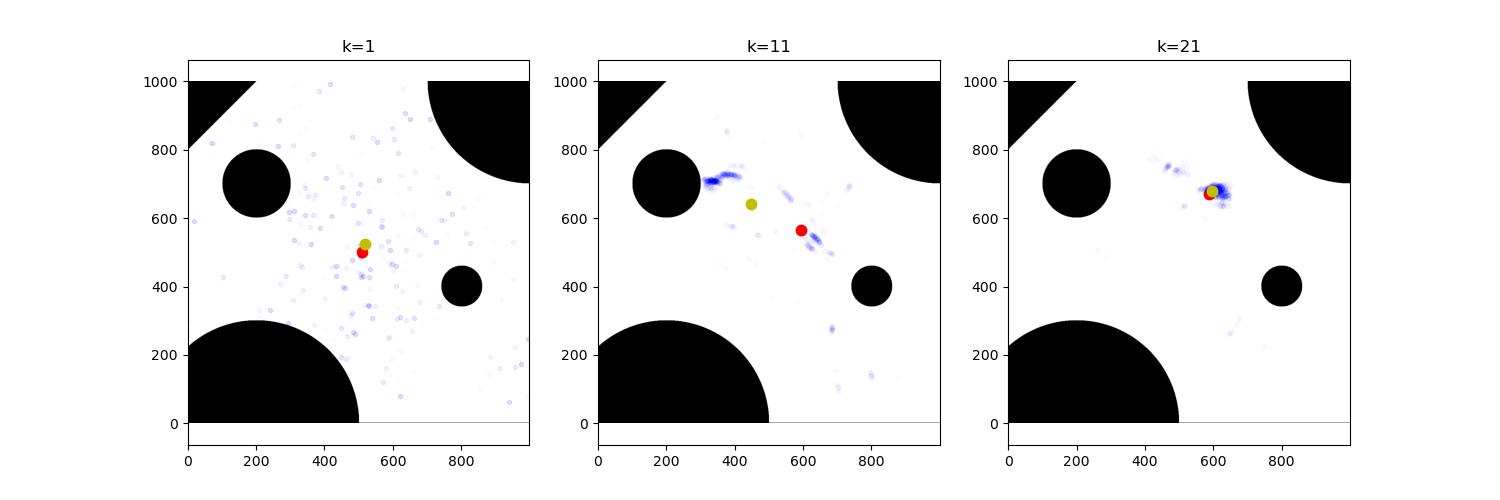
\includegraphics[width=15cm]{./mersenne_example.png}
		\caption{Przykładowe wyniki dla generatora Mersenne Twister}
		\label{mersenne_example}
	\end{center}
\end{figure}

\begin{figure}[H]
\begin{center}
	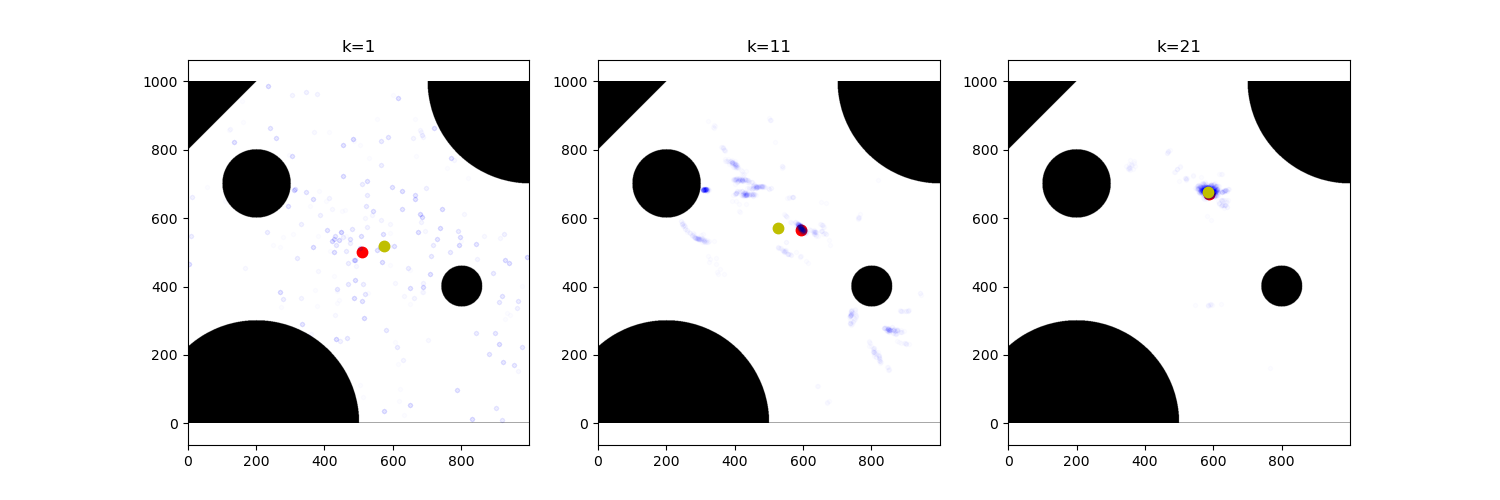
\includegraphics[width=15cm]{./device_example.png}
	\caption{Przykładowe wyniki dla niedeterministycznego generatora}
	\label{device_example}
\end{center}
\end{figure}


\subsection{Niejednoznaczna mapa}
W tym przypadku zbadano jak zachowa się filtr przy braku punktów odniesienia. W kwadratowym pokoju, powinno to spowodować pojawienie się czterech równie prawdopodobnych pozycji. Jak widać przewidywania potwierdziły się na rysunku \ref{no_pivot}. Na rysunku \ref{one_pivot} przedstawiono sytuację, gdy mapa dopuszcza dwie możliwe pozycja. Badania przeprowadzono przy populacji $N=10000$ cząstek.

\begin{figure}[H]
	\begin{center}
		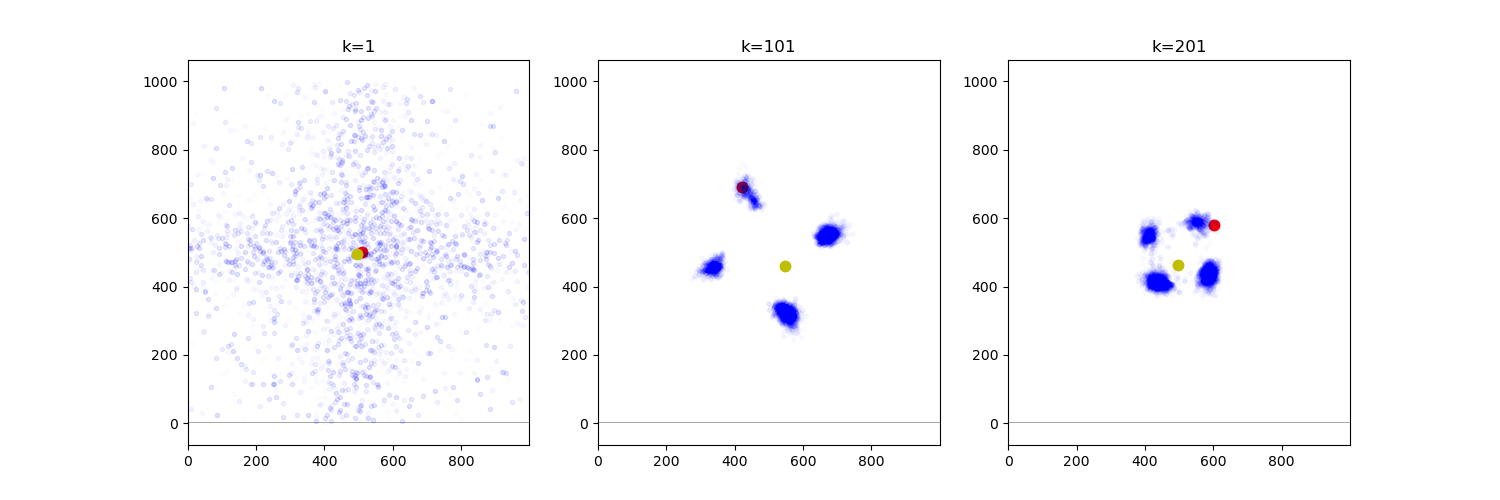
\includegraphics[width=15cm]{./no_pivot.png}
		\caption{Przykładowe wyniki przy braku punktu odniesienia}
		\label{no_pivot}
	\end{center}
\end{figure}

\begin{figure}[H]
	\begin{center}
		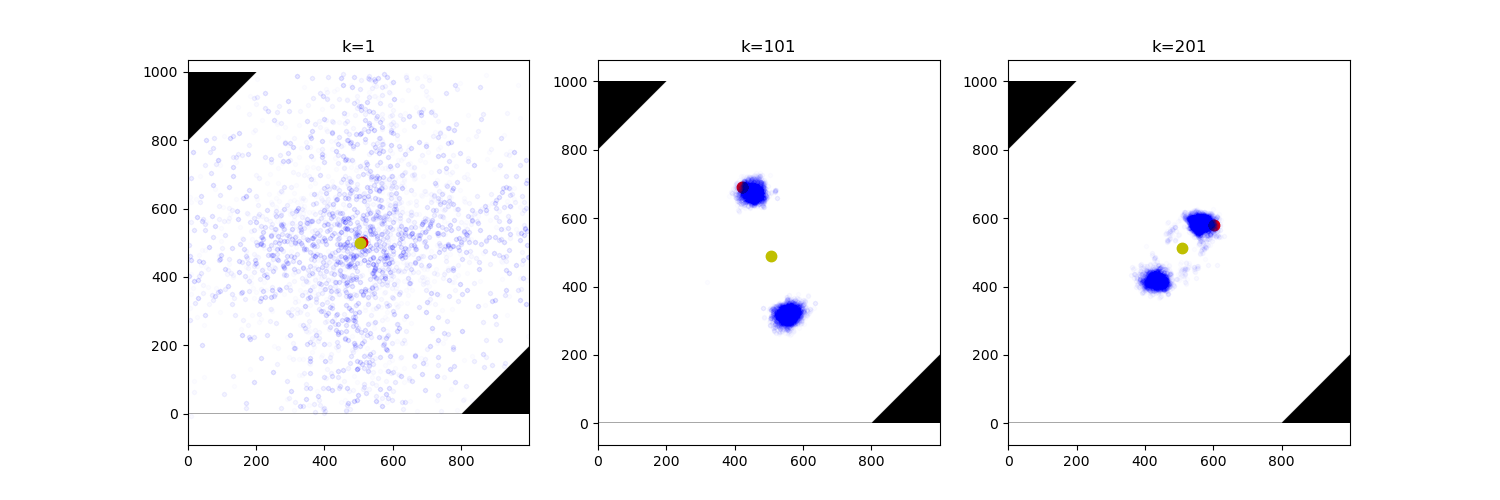
\includegraphics[width=15cm]{./one_pivot.png}
		\caption{Przykładowe wyniki przy dwóch możliwych położeniach}
		\label{one_pivot}
	\end{center}
\end{figure}

\subsection{Brak ewolucji systemu}
Tutaj Zbadano, co się dzieje, gdy system nie ewoluuje. Spodziewano się, pojawią się izohipsy, przynajmniej na początku, nim populacja nie stanie się zbyt zdegenerowana. Badania przeprowadzono dla populacji o rozmiarze $N=100000$. Jak widać na rysunkach \ref{stationary} i \ref{stationary_plane} przewidywania się spełniły, dodatkowo dla rysunku \ref{stationary_plane} dobrze widać problem się degeneracji. Problem ten można rozwiązać dzięki podejściu z rozdziału \ref{evol_chap}, które zademonstrowano na rysunku \ref{stationary_evol}, na którym widać jakwychwycone zostały obszary na tej samej wysokości.

\begin{figure}[H]
	\begin{center}
		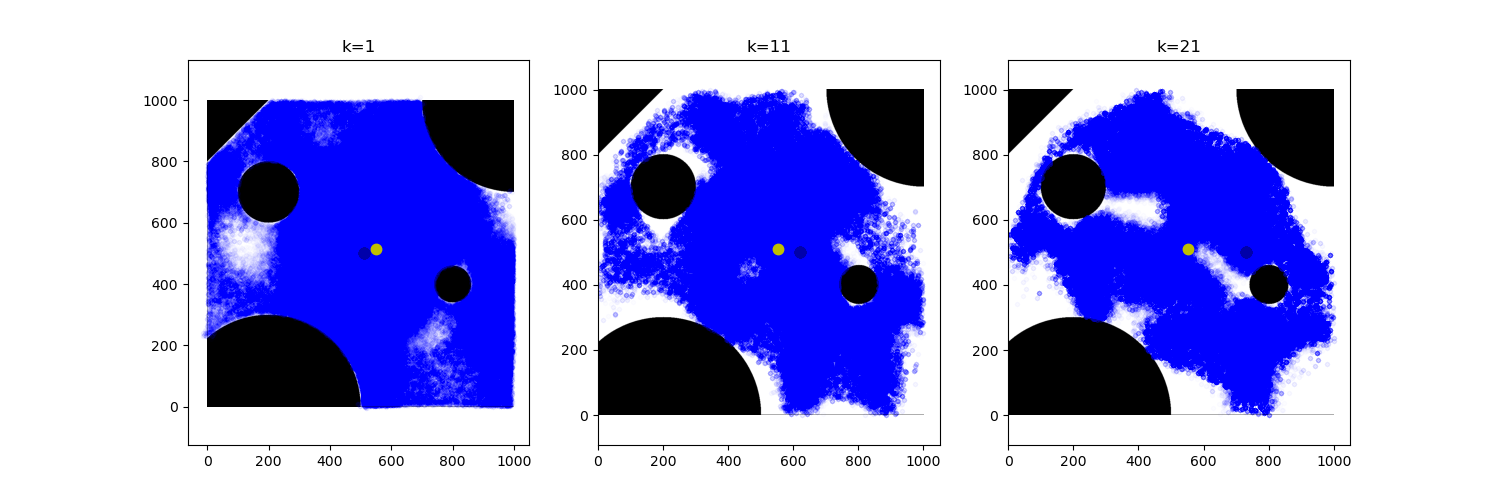
\includegraphics[width=15cm]{./stationary.png}
		\caption{Przykładowe wyniki przy braku ewolucji systemu, dla robota w pokoju.}
		\label{stationary}
	\end{center}
\end{figure}

\begin{figure}[H]
\begin{center}
	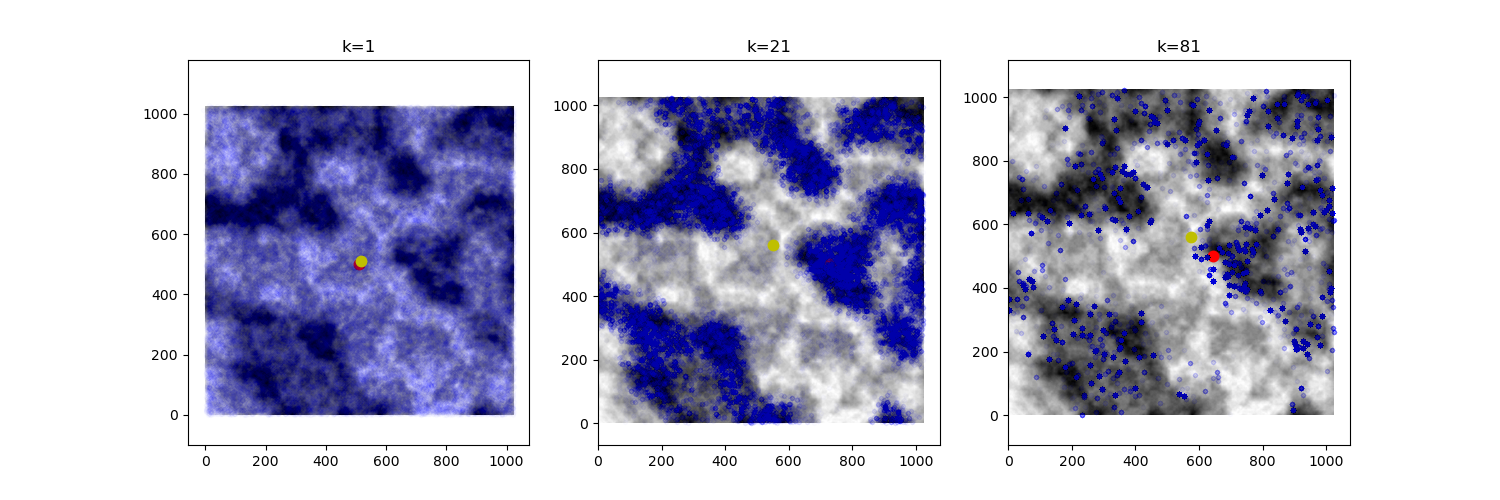
\includegraphics[width=15cm]{./stationary_plane.png}
	\caption{Przykładowe wyniki przy braku ewolucji systemu, dla samolotu.}
	\label{stationary_plane}
\end{center}
\end{figure}

\begin{figure}[H]
	\begin{center}
		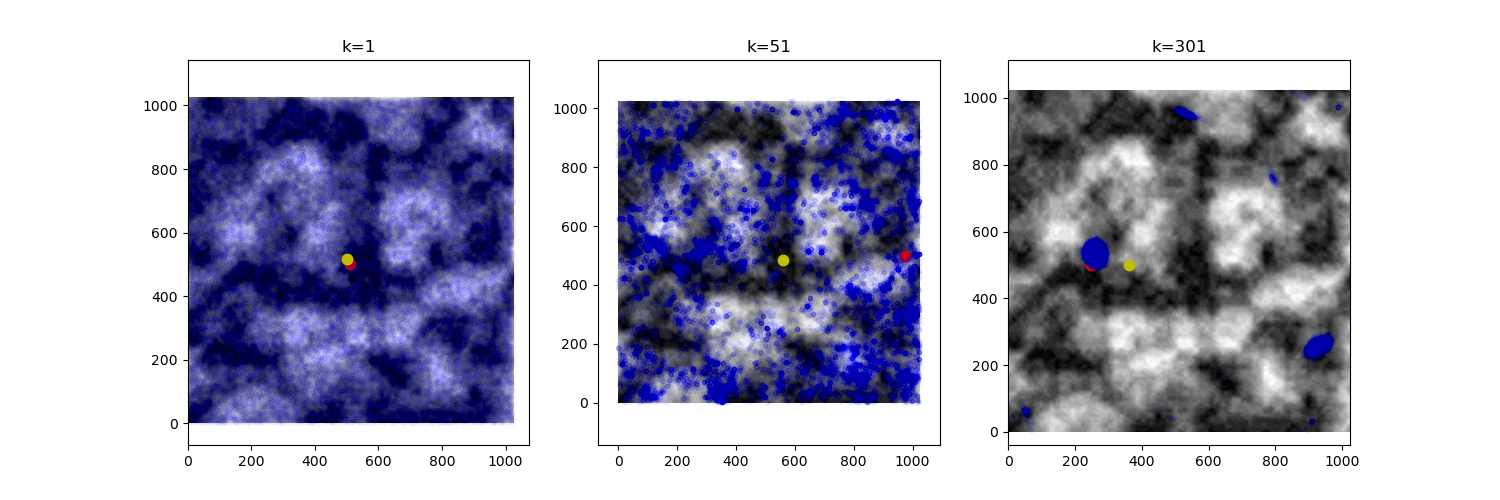
\includegraphics[width=15cm]{./stationary_evol.png}
		\caption{Przykładowe wyniki przy braku ewolucji systemu, dla samolotu, przy zmodyfikowanym algorytmie}
		\label{stationary_evol}
	\end{center}
\end{figure}


%\subsection{Pomiary bez związku}
%powinien pozostać jednostajny szum

\section{Wpływ sposobu estymowania położenia}
Przebadano trzy metody estymowania położenia: średnią ważoną cząstek, średnią ważoną 10\% najlepszych cząstek, najlepszą cząstkę. Badania przeprowadzono na populacji 300 cząstek. Na wykresie \ref{wplyw_est} przedstawiono wyniki, z których wynika, że między średnią ważoną z najlepszych 10\% i i najlepszym osobnikiem.

\begin{figure}[H]
	\begin{center}
		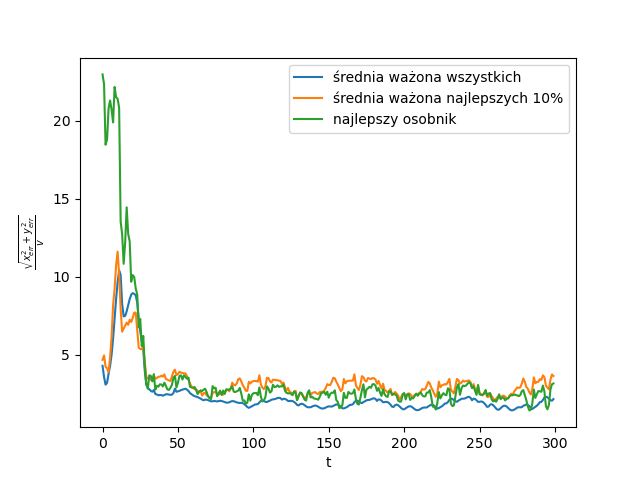
\includegraphics[width=12cm]{./wplyw_est.png}
		\caption{Przykładowe wyniki przy braku ewolucji systemu, dla samolotu}
		\label{wplyw_est}
	\end{center}
\end{figure}

%\section{Wpływ funkcji określającej błąd pomiaru}

\section{Wpływ liczby cząstek}
Zbadano wpływ liczby cząstek na jakość estymacji. Badania przeprowadzono dla  robota w pokoju, dla czterech różnych $N$, 100, 300, 1000 i 10000, wyniki uśredniając po 100 razy. Wyniki zestawiono na rysunku \ref{wplyw_N}. Jako błąd przyjęto pierwiastek sumy kwadratów błędów w kierunkach $x$ i $y$, podzielony przez prędkość rzeczywistego robota. Jak widać, wraz ze wzrostem cząstek poprawia się jakość estymacji, jednak dzieje się tak do pewnego momentu, po którym zwiększenie liczb cząstek nie poprawia jakości estymacji (tutaj wyniosła ona około 1000 cząstek). Na wykresie \ref{dynamic_N} widać jak zmieniała się liczba cząstek, gdy zastosowano podejście opisane w rozdziale \ref{adaptive_chapter}. Wartości parametrów ustalono następująco: $N_{min}=100, N_{max}=1000, \alpha = 50, \gamma = 1$.  Jak widać nie tracąc za bardzo na jakości estymacji można znacząco zredukować liczbę cząstek.

\begin{figure}[H]
	\begin{center}
		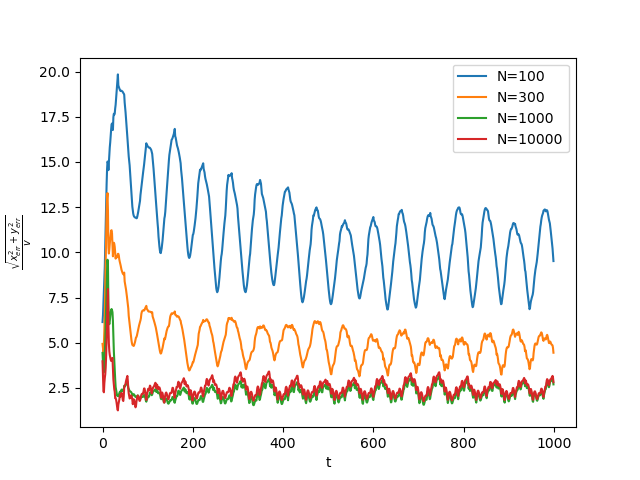
\includegraphics[width=12cm]{./wplyw_N.png}
		\caption{Wpływ liczby cząstek na jakość estymacji dla robota w pokoju.}
		\label{wplyw_N}
	\end{center}
\end{figure}

\begin{figure}[H]
	\begin{center}
		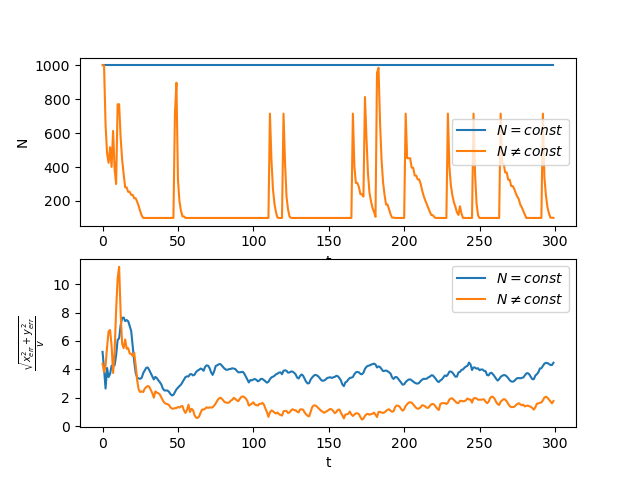
\includegraphics[width=12cm]{./dynamic_N.png}
		\caption{Wpływ dynamicznej zmiany liczby cząstek na jakość estymacji dla robota w pokoju.}
		\label{dynamic_N}
	\end{center}
\end{figure}

\section{Wpływ szumu}

\begin{figure}[H]
	\begin{center}
		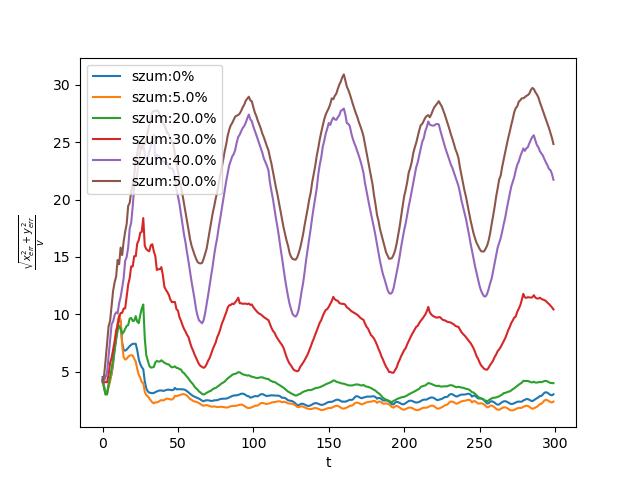
\includegraphics[width=12cm]{./wplyw_szumu.png}
		\caption{Wpływ zaszumienia pomiaru na jakość estymacji dla robota w pokoju.}
		\label{wplyw_szumu}
	\end{center}
\end{figure}
\begin{figure}[H]
\begin{center}
	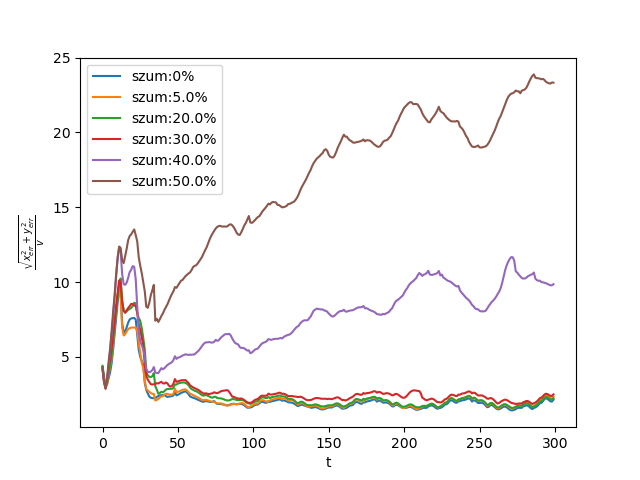
\includegraphics[width=12cm]{./wplyw_szumu_ori.png}
	\caption{Wpływ zaszumienia odczytu zmiany orientacji na jakość estymacji dla robota w pokoju.}
	\label{wplyw_szumu_ori}
\end{center}
\end{figure}

\begin{figure}[H]
	\begin{center}
		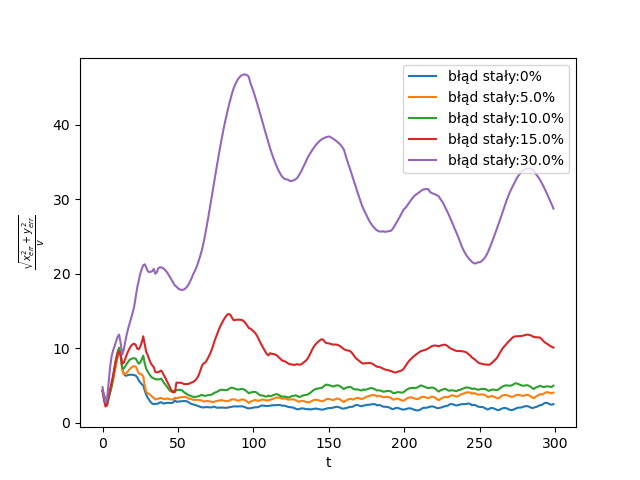
\includegraphics[width=12cm]{./blad_staly.png}
		\caption{Wpływ pojawienia się błędu stałego na jakość estymacji dla robota w pokoju.}
		\label{blad_staly}
	\end{center}
\end{figure}

\section{Wpływ metody próbkowania}
Przebadano dwie metody próbkowania: najpopularniejszy stochastic universal sampling \cite{sus_wiki} (SUS), z którego się korzysta ze względu na niską złożoność obliczeniową, oraz roulette sampling \cite{rou_wiki}. Badania przeprowadzono dla trzech różnych rozmiarów populacji: 100,300,1000, wyniki uśredniając po 100 razy. Jak widać, SUS daje zazwyczaj lepsze wyniki, zwłaszcza dla niewielkich populacji. 

\begin{figure}[H]
	\begin{center}
		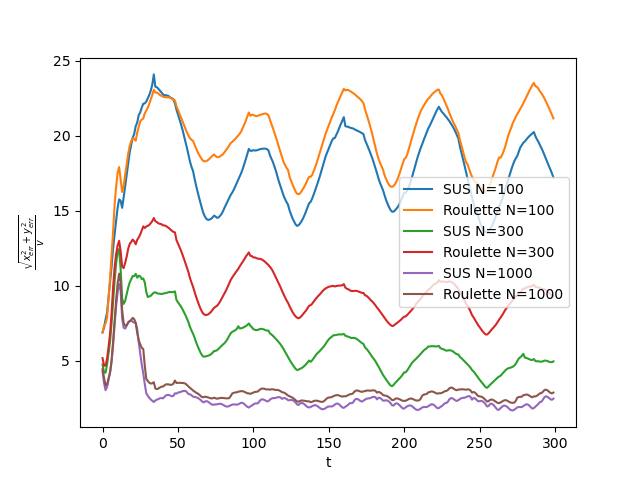
\includegraphics[width=12cm]{./sampling_impact.png}
		\caption{Wpływ metody próbkowania cząstek na jakość estymacji.}
		\label{sampling_impact}
	\end{center}
\end{figure}


\section{Skuteczność w poprawianiu błędnie określonego położenia}
Sprawdzono zachowanie filtra w sytuacji, gdy w jakiś sposób nie poradzi sobie o określeniem położenia, i zgubi się. Wyniki widać na rysunku \ref{lost}. Można zaobserwować, iż algorytm jest w stanie "odszukać" faktyczny stan, jednak jest to bardziej kwestia szczęścia. Podejście opisane w rozdziale \ref{evol_chap} jest w stanie delikatnie poprawić rozwiązanie, jednak nie jest ono tak skuteczne jak przeszukanie od nowa całej przestrzeni stanów jak to się robi w przypadku algorytmu opisanego w rozdziale \ref{bpf_chapter}.
\begin{figure}[H]
	\begin{center}
		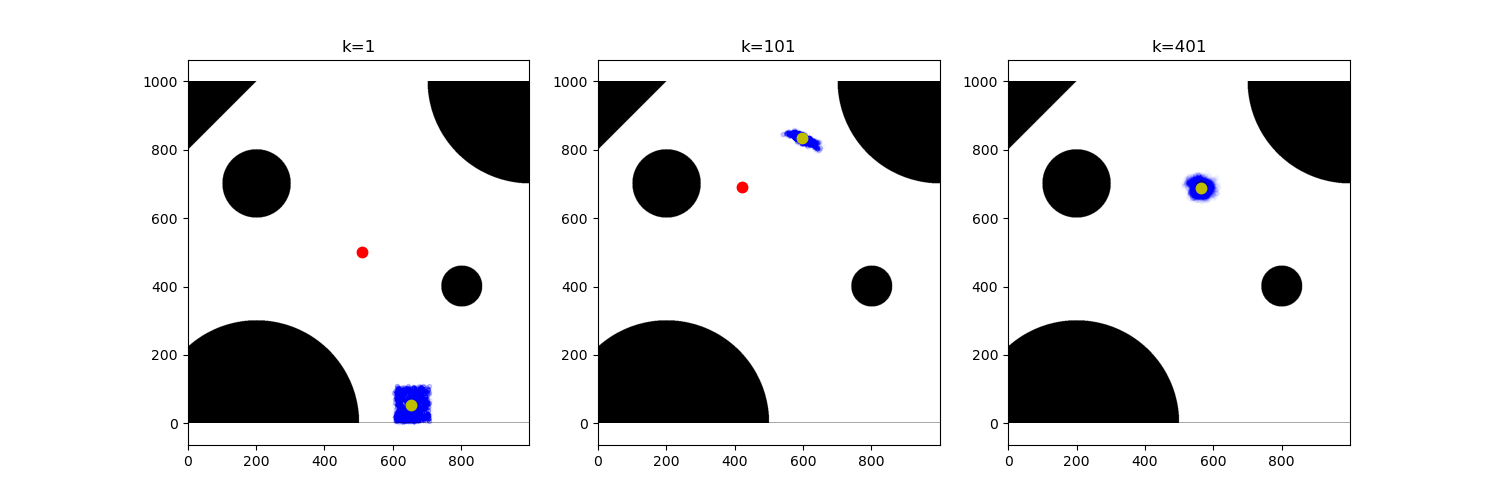
\includegraphics[width=15cm]{./lost.png}
		\caption{Sprawdzenie jak filtr radzi sobie w sytuacji gdy nie ma cząstek w pobliży faktycznego stanu.}
		\label{lost}
	\end{center}
\end{figure}
\begin{figure}[H]
\begin{center}
	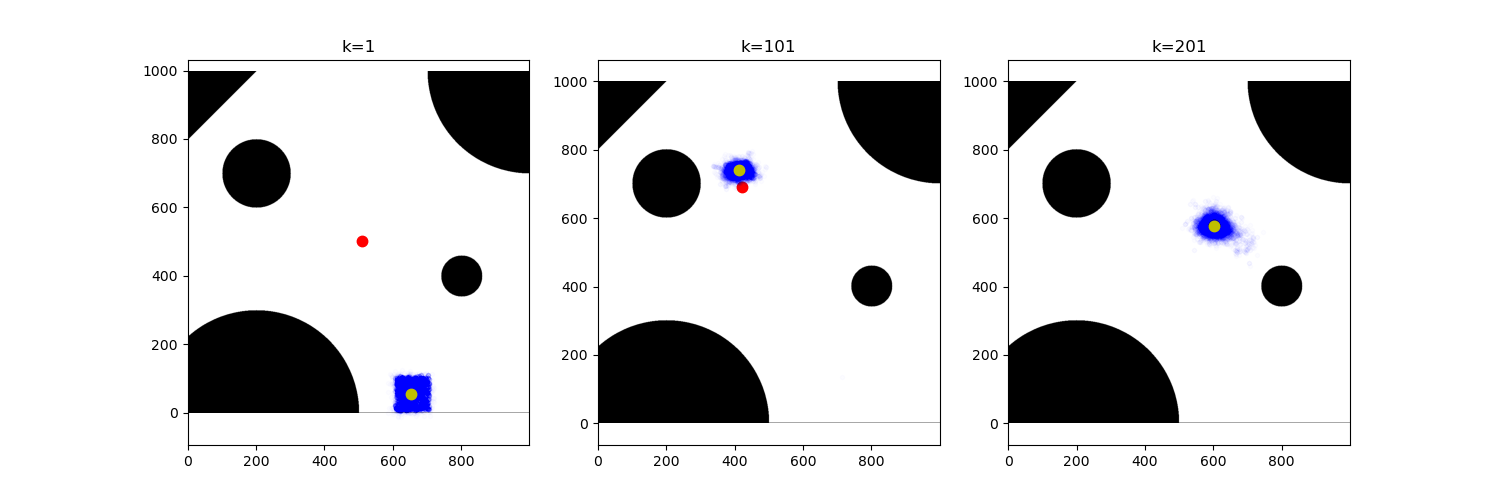
\includegraphics[width=15cm]{./lost_evol.png}
	\caption{Sprawdzenie jak zmodyfikowany filtr radzi sobie w sytuacji gdy nie ma cząstek w pobliży faktycznego stanu.}
	\label{lost_evol}
\end{center}
\end{figure}
\section{Wpływ różnorodności terenu}
\section{Rozkład p przy dryfie - chodzi o genetyczne}

